\chapter{Quadrature Amplitude Modulation (QAM)}
\label{ch:qam}

\begin{nontechnical}
\textbf{QAM is like having a grid of mailboxes}---the more boxes, the more messages you can send at once. Your WiFi router picks bigger grids when signal is strong!

\textbf{The idea---vary BOTH brightness and angle:}
\begin{itemize}
\item \textbf{PSK} (like QPSK): Only varies angle (4 or 8 positions)
\item \textbf{QAM}: Varies \textbf{both} angle AND distance from center
\item Result: Many more possible positions = much faster data
\end{itemize}

\textbf{Real QAM sizes:}
\begin{itemize}
\item \textbf{16-QAM}: $4 \times 4$ grid = 16 positions = 4 bits/symbol
\item \textbf{64-QAM}: $8 \times 8$ grid = 64 positions = 6 bits/symbol
\item \textbf{256-QAM}: $16 \times 16$ grid = 256 positions = 8 bits/symbol
\item \textbf{1024-QAM} (WiFi 6): $32 \times 32$ grid = 1024 positions = 10 bits/symbol
\end{itemize}

\textbf{The trade-off:} More positions = faster, BUT positions are closer together and easier to confuse when signal is noisy. Strong signal (close to router): use 1024-QAM. Weak signal (far from router): use QPSK.

\textbf{Fun fact:} Modern WiFi 6E can use 1024-QAM, but ONLY at close range with zero interference---it's like threading a needle with radio waves!
\end{nontechnical}

\section{Overview}

\textbf{Quadrature Amplitude Modulation (QAM)} is a digital modulation scheme that encodes data by modulating \textbf{both the amplitude and phase} of a carrier wave, achieving optimal use of the two-dimensional signal space.

\begin{keyconcept}
QAM provides the \textbf{highest spectral efficiency} of any modulation scheme for a given signal-to-noise ratio by combining amplitude-shift keying (ASK) and phase-shift keying (PSK) in the I/Q plane. This makes it the dominant choice for modern broadband systems including WiFi, LTE/5G, cable modems, and microwave backhaul.
\end{keyconcept}

QAM extends naturally from QPSK (which is actually 4-QAM) to higher-order constellations such as 16-QAM, 64-QAM, 256-QAM, and beyond, trading increased data rate for higher SNR requirements.

\section{Mathematical Description}

\subsection{Complex Baseband Representation}

The M-ary QAM signal can be expressed in complex baseband form as:
\begin{equation}
s_m = I_m + jQ_m
\label{eq:qam-baseband}
\end{equation}
where:
\begin{itemize}
\item $I_m$ = In-phase amplitude (real axis)
\item $Q_m$ = Quadrature amplitude (imaginary axis)
\item $m$ = Symbol index ($0$ to $M-1$)
\item $M$ = constellation size (number of symbols)
\end{itemize}

\subsection{Time-Domain Signal}

The passband QAM waveform is:
\begin{equation}
s(t) = I_m \cos(2\pi f_c t) - Q_m \sin(2\pi f_c t)
\label{eq:qam-passband}
\end{equation}
where:
\begin{itemize}
\item $f_c$ = carrier frequency (Hz)
\item $I_m, Q_m$ = symbol amplitudes from constellation
\item Symbol duration = $T_s$ seconds
\end{itemize}

\textbf{Alternative representation:}
\begin{equation}
s(t) = A_m \cos(2\pi f_c t + \phi_m)
\end{equation}
where $A_m = \sqrt{I_m^2 + Q_m^2}$ (amplitude) and $\phi_m = \arctan(Q_m/I_m)$ (phase).

\begin{keyconcept}
Unlike PSK (constant amplitude, variable phase) or ASK (variable amplitude, fixed phase), QAM modulates \textbf{both amplitude and phase simultaneously}, creating a rectangular constellation in the I/Q plane that maximizes the minimum Euclidean distance between symbols for a given average power.
\end{keyconcept}

\subsection{M-ary QAM}

For square QAM constellations:
\begin{equation}
M = 2^k \quad\text{where}\quad k = \log_2(M)
\end{equation}

\textbf{Bits per symbol:} $k = \log_2(M)$

\textbf{Typical values:}
\begin{itemize}
\item $M = 4$ (QPSK): $k = 2$ bits/symbol
\item $M = 16$ (16-QAM): $k = 4$ bits/symbol
\item $M = 64$ (64-QAM): $k = 6$ bits/symbol
\item $M = 256$ (256-QAM): $k = 8$ bits/symbol
\item $M = 1024$ (1024-QAM): $k = 10$ bits/symbol
\item $M = 4096$ (4096-QAM): $k = 12$ bits/symbol
\end{itemize}

For square QAM, the constellation forms a $\sqrt{M} \times \sqrt{M}$ grid in the I/Q plane.

\section{Constellation Diagrams}

QAM constellations are visualized as grids in the I/Q plane, with symbol positions determined by discrete amplitude levels on both axes.

\begin{center}
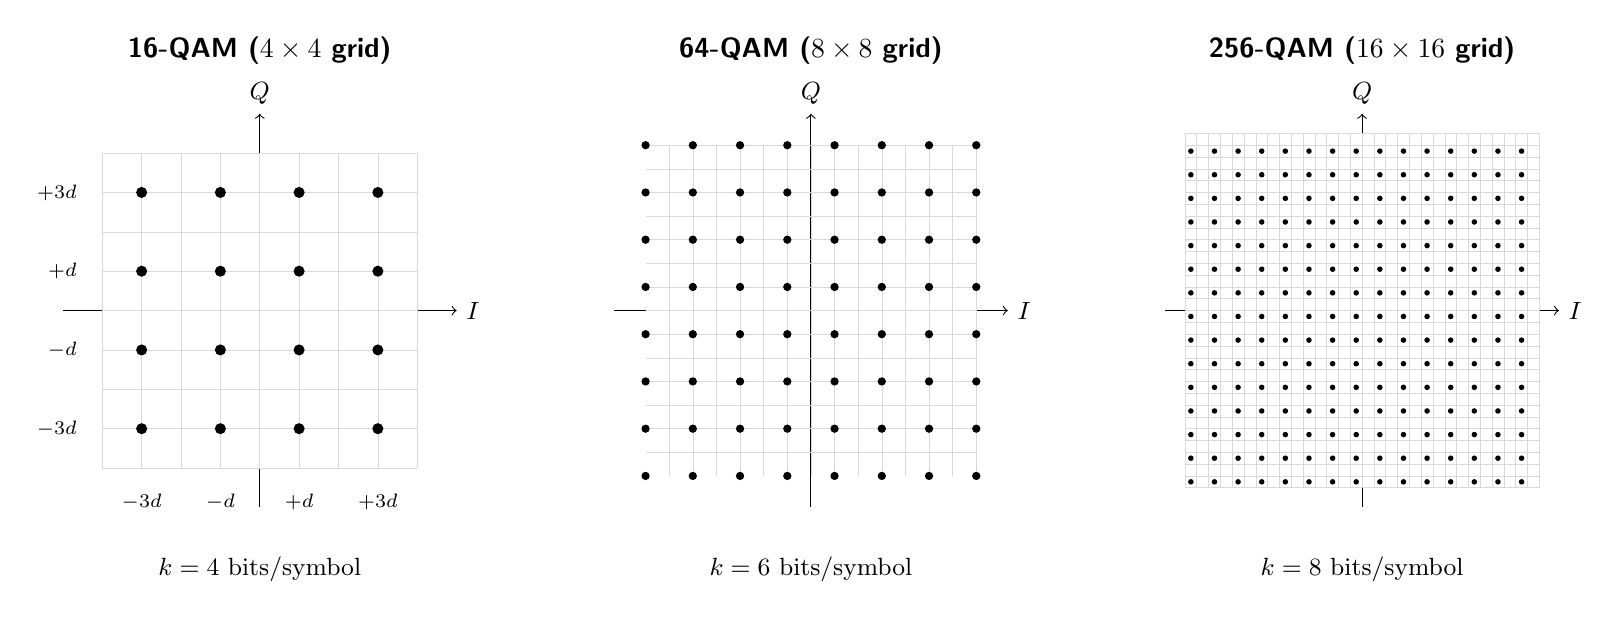
\begin{tikzpicture}[scale=1.0]
% 16-QAM
\begin{scope}[shift={(0,0)}]
\node[above,font=\sffamily\bfseries] at (0,3) {16-QAM ($4 \times 4$ grid)};
\draw[->] (-2.5,0) -- (2.5,0) node[right,font=\sffamily\small] {$I$};
\draw[->] (0,-2.5) -- (0,2.5) node[above,font=\sffamily\small] {$Q$};
\draw[very thin,gray!30] (-2,-2) grid[step=0.5] (2,2);

% 16-QAM constellation points
\foreach \i in {-1.5,-0.5,0.5,1.5} {
  \foreach \q in {-1.5,-0.5,0.5,1.5} {
    \fill[black] (\i,\q) circle (2pt);
  }
}

% Labels for amplitude levels
\node[below,font=\scriptsize] at (-1.5,-2.2) {$-3d$};
\node[below,font=\scriptsize] at (-0.5,-2.2) {$-d$};
\node[below,font=\scriptsize] at (0.5,-2.2) {$+d$};
\node[below,font=\scriptsize] at (1.5,-2.2) {$+3d$};
\node[left,font=\scriptsize] at (-2.2,-1.5) {$-3d$};
\node[left,font=\scriptsize] at (-2.2,-0.5) {$-d$};
\node[left,font=\scriptsize] at (-2.2,0.5) {$+d$};
\node[left,font=\scriptsize] at (-2.2,1.5) {$+3d$};

\node[below,font=\small] at (0,-3) {$k = 4$ bits/symbol};
\end{scope}

% 64-QAM
\begin{scope}[shift={(7,0)}]
\node[above,font=\sffamily\bfseries] at (0,3) {64-QAM ($8 \times 8$ grid)};
\draw[->] (-2.5,0) -- (2.5,0) node[right,font=\sffamily\small] {$I$};
\draw[->] (0,-2.5) -- (0,2.5) node[above,font=\sffamily\small] {$Q$};
\draw[very thin,gray!30] (-2.1,-2.1) grid[step=0.3] (2.1,2.1);

% 64-QAM constellation points (8x8 grid)
\foreach \i in {-2.1,-1.5,-0.9,-0.3,0.3,0.9,1.5,2.1} {
  \foreach \q in {-2.1,-1.5,-0.9,-0.3,0.3,0.9,1.5,2.1} {
    \fill[black] (\i,\q) circle (1.5pt);
  }
}

\node[below,font=\small] at (0,-3) {$k = 6$ bits/symbol};
\end{scope}

% 256-QAM
\begin{scope}[shift={(14,0)}]
\node[above,font=\sffamily\bfseries] at (0,3) {256-QAM ($16 \times 16$ grid)};
\draw[->] (-2.5,0) -- (2.5,0) node[right,font=\sffamily\small] {$I$};
\draw[->] (0,-2.5) -- (0,2.5) node[above,font=\sffamily\small] {$Q$};
\draw[very thin,gray!30] (-2.25,-2.25) grid[step=0.15] (2.25,2.25);

% 256-QAM constellation points (16x16 grid - subset for clarity)
\foreach \i in {-2.175,-1.875,...,2.175} {
  \foreach \q in {-2.175,-1.875,...,2.175} {
    \fill[black] (\i,\q) circle (1pt);
  }
}

\node[below,font=\small] at (0,-3) {$k = 8$ bits/symbol};
\end{scope}
\end{tikzpicture}
\end{center}

\subsection{16-QAM Constellation Details}

The 16-QAM constellation consists of a $4 \times 4$ grid in the I/Q plane:

\textbf{Amplitude levels:} $I, Q \in \{-3d, -d, +d, +3d\}$

where $d$ is the unit spacing (normalized distance between adjacent symbols).

\subsection{Gray Coding}

To minimize bit errors when symbols are misdetected, QAM uses \textbf{Gray coding}, where adjacent constellation points differ by only one bit.

For 16-QAM with 4 bits per symbol ($b_3 b_2 b_1 b_0$):
\begin{itemize}
\item $b_3 b_2$ $\rightarrow$ I component: $00 = -3d$, $01 = -d$, $11 = +d$, $10 = +3d$
\item $b_1 b_0$ $\rightarrow$ Q component: $00 = -3d$, $01 = -d$, $11 = +d$, $10 = +3d$
\end{itemize}

\begin{center}
\begin{tabular}{@{}cccc@{}}
\toprule
Bits & $I$ & $Q$ & Position \\
\midrule
0000 & $-3d$ & $-3d$ & Bottom-left corner \\
0001 & $-3d$ & $-d$ & \\
0011 & $-3d$ & $+d$ & \\
0010 & $-3d$ & $+3d$ & Top-left corner \\
1010 & $+3d$ & $+3d$ & Top-right corner \\
1011 & $+3d$ & $+d$ & \\
1001 & $+3d$ & $-d$ & \\
1000 & $+3d$ & $-3d$ & Bottom-right corner \\
\bottomrule
\end{tabular}
\end{center}

\begin{keyconcept}
Gray coding ensures that the most probable errors (to adjacent constellation points) result in only a single bit error rather than multiple bit errors. This reduces the average bit error rate by approximately a factor of $\log_2(M)$.
\end{keyconcept}

\subsection{Signal Energy and Normalization}

\subsubsection{Average Symbol Energy (16-QAM)}

The average symbol energy for 16-QAM is:
\begin{equation}
\bar{E}_s = \frac{1}{16}\sum_{m=0}^{15} (I_m^2 + Q_m^2) = \frac{1}{16} \times 16 \times 10d^2 = 10d^2
\label{eq:qam16-energy}
\end{equation}

\textbf{Calculation:} Each of the 16 symbols has energy $I_m^2 + Q_m^2$. For $I, Q \in \{-3d, -d, +d, +3d\}$:
\begin{itemize}
\item Corner symbols: $(3d)^2 + (3d)^2 = 18d^2$ (4 symbols)
\item Edge symbols: $(3d)^2 + (d)^2 = 10d^2$ or $(d)^2 + (3d)^2 = 10d^2$ (8 symbols)
\item Inner symbols: $(d)^2 + (d)^2 = 2d^2$ (4 symbols)
\item Average: $(4 \times 18 + 8 \times 10 + 4 \times 2)/16 = 160/16 = 10d^2$
\end{itemize}

\textbf{Normalization:} Setting $d^2 = 1/10$ gives $\bar{E}_s = 1$.

\subsubsection{Minimum Euclidean Distance}

The minimum distance between adjacent symbols is:
\begin{equation}
d_{\min} = 2d
\label{eq:qam-dmin}
\end{equation}

With normalization ($d = 1/\sqrt{10}$):
\begin{equation}
d_{\min} = \frac{2}{\sqrt{10}} = 0.632
\end{equation}

This determines the noise immunity---larger $d_{\min}$ provides better BER performance.

\section{Modulation and Demodulation}

\subsection{QAM Modulator}

The QAM modulator uses a standard I/Q architecture identical to QPSK, but with multi-level symbol mapping:

\begin{center}
\begin{tikzpicture}[
  block/.style={rectangle, draw, minimum width=2.2cm, minimum height=1cm, font=\sffamily\small},
  node distance=2.2cm,
  font=\small
]
\node (input) {\sffamily Binary\\Data};
\node[block, right of=input, node distance=2.8cm] (mapper) {Symbol\\Mapper};
\node[block, above right of=mapper, node distance=2.8cm] (daci) {DAC};
\node[block, below right of=mapper, node distance=2.8cm] (dacq) {DAC};
\node[block, right of=daci, node distance=2.8cm] (multi) {Mixer\\$\times$};
\node[block, right of=dacq, node distance=2.8cm] (multq) {Mixer\\$\times$};
\node[circle, draw, right of=multi, node distance=2.8cm, minimum size=0.8cm] (sum) {$+$};
\node[block, right of=sum, node distance=2.5cm] (filter) {Bandpass\\Filter};
\node[right of=filter, node distance=2.8cm] (output) {\sffamily QAM\\Output};

\node[above of=multi, node distance=1.5cm, font=\scriptsize] (cos) {$\cos(2\pi f_c t)$};
\node[below of=multq, node distance=1.5cm, font=\scriptsize] (sin) {$-\sin(2\pi f_c t)$};

\draw[->,thick] (input) -- (mapper);
\draw[->,thick] (mapper) -- node[above,font=\scriptsize,sloped] {$I_m$} (daci);
\draw[->,thick] (mapper) -- node[below,font=\scriptsize,sloped] {$Q_m$} (dacq);
\draw[->,thick] (daci) -- (multi);
\draw[->,thick] (dacq) -- (multq);
\draw[->,thick] (cos) -- (multi);
\draw[->,thick] (sin) -- (multq);
\draw[->,thick] (multi) -- (sum);
\draw[->,thick] (multq) -- (sum);
\draw[->,thick] (sum) -- (filter);
\draw[->,thick] (filter) -- (output);
\end{tikzpicture}
\end{center}

\textbf{Process:}
\begin{enumerate}
\item \textbf{Symbol mapping:} Map $k = \log_2(M)$ bits to constellation point $(I_m, Q_m)$ using Gray coding
\item \textbf{Digital-to-analog conversion:} Generate analog I and Q waveforms
\item \textbf{Quadrature modulation:} 
  \begin{itemize}
  \item I channel: Multiply by $\cos(2\pi f_c t)$
  \item Q channel: Multiply by $-\sin(2\pi f_c t)$
  \end{itemize}
\item \textbf{Summation:} Combine to form $s(t) = I_m \cos(2\pi f_c t) - Q_m \sin(2\pi f_c t)$
\item \textbf{Pulse shaping:} Apply bandpass filter (raised-cosine) to limit bandwidth
\end{enumerate}

\subsection{Coherent QAM Demodulator}

\begin{center}
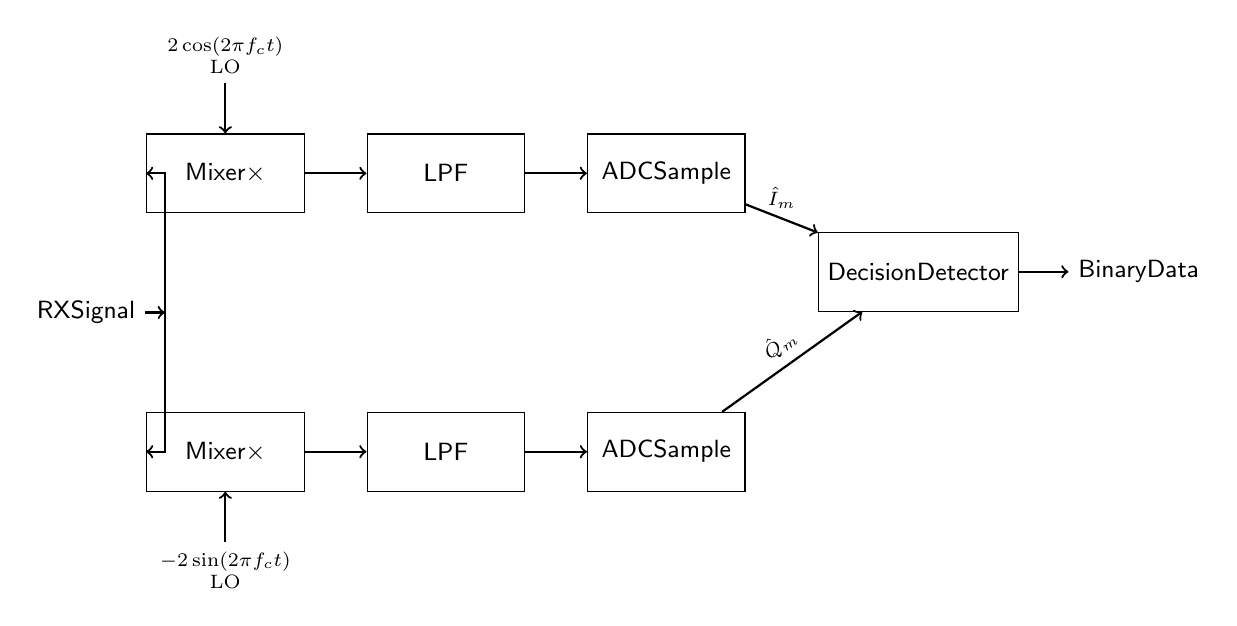
\begin{tikzpicture}[
  block/.style={rectangle, draw, minimum width=2cm, minimum height=1cm, font=\sffamily\small},
  node distance=2cm,
  font=\small
]
\node (input) {\sffamily RX\\Signal};
\node[block, above right of=input, node distance=2.5cm] (multi) {Mixer\\$\times$};
\node[block, below right of=input, node distance=2.5cm] (multq) {Mixer\\$\times$};
\node[block, right of=multi, node distance=2.8cm] (lpfi) {LPF};
\node[block, right of=multq, node distance=2.8cm] (lpfq) {LPF};
\node[block, right of=lpfi, node distance=2.8cm] (adci) {ADC\\Sample};
\node[block, right of=lpfq, node distance=2.8cm] (adcq) {ADC\\Sample};
\node[block, right of=adci, node distance=3.2cm, yshift=-1.25cm] (decision) {Decision\\Detector};
\node[right of=decision, node distance=2.8cm] (output) {\sffamily Binary\\Data};

\node[above of=multi, node distance=1.5cm, font=\scriptsize, align=center] (loi) {$2\cos(2\pi f_c t)$\\LO};
\node[below of=multq, node distance=1.5cm, font=\scriptsize, align=center] (loq) {$-2\sin(2\pi f_c t)$\\LO};

\draw[->,thick] (input) -- ++(1,0) coordinate(split);
\draw[->,thick] (split) |- (multi);
\draw[->,thick] (split) |- (multq);
\draw[->,thick] (loi) -- (multi);
\draw[->,thick] (loq) -- (multq);
\draw[->,thick] (multi) -- node[above,font=\scriptsize] {} (lpfi);
\draw[->,thick] (multq) -- node[above,font=\scriptsize] {} (lpfq);
\draw[->,thick] (lpfi) -- node[above,font=\scriptsize] {} (adci);
\draw[->,thick] (lpfq) -- node[above,font=\scriptsize] {} (adcq);
\draw[->,thick] (adci) -- node[above,font=\scriptsize] {$\hat{I}_m$} (decision);
\draw[->,thick] (adcq) -- node[above,font=\scriptsize,sloped] {$\hat{Q}_m$} (decision);
\draw[->,thick] (decision) -- (output);
\end{tikzpicture}
\end{center}

\textbf{Detection process:}
\begin{enumerate}
\item \textbf{Quadrature downconversion:} Multiply received signal by in-phase and quadrature local oscillators
\item \textbf{Lowpass filtering:} Remove double-frequency ($2f_c$) components
\item \textbf{Sampling:} Sample at symbol rate $1/T_s$ to obtain $\hat{I}_m$ and $\hat{Q}_m$
\item \textbf{Minimum distance detection:} Find constellation point $(I_m, Q_m)$ closest to $(\hat{I}_m, \hat{Q}_m)$
\item \textbf{Symbol demapping:} Convert constellation point to $k$ bits using inverse Gray mapping
\end{enumerate}

\begin{warningbox}
\textbf{Phase synchronization is critical.} The local oscillator must be exactly in phase with the transmitter carrier. A phase offset $\phi_e$ causes constellation rotation, reducing the effective distance between symbols and increasing BER. Phase errors $> 5°$ significantly degrade high-order QAM (256-QAM, 1024-QAM).
\end{warningbox}

\section{Higher-Order QAM}

\subsection{64-QAM}

The 64-QAM constellation consists of an $8 \times 8$ grid:

\textbf{Amplitude levels:} $I, Q \in \{-7d, -5d, -3d, -d, +d, +3d, +5d, +7d\}$

\textbf{Bits per symbol:} $k = 6$

\textbf{Average energy:}
\begin{equation}
\bar{E}_s = \frac{1}{64}\sum_{m=0}^{63} (I_m^2 + Q_m^2) = 42d^2
\end{equation}

\textbf{Normalized:} $d = 1/\sqrt{42}$ gives $\bar{E}_s = 1$

\textbf{Minimum distance:} $d_{\min} = 2d = 2/\sqrt{42} = 0.309$

\subsection{256-QAM}

The 256-QAM constellation forms a $16 \times 16$ grid:

\textbf{Bits per symbol:} $k = 8$

\textbf{Average energy:} $\bar{E}_s = 170d^2$

\textbf{Normalized:} $d = 1/\sqrt{170}$ gives $\bar{E}_s = 1$

\textbf{Minimum distance:} $d_{\min} = 2d = 2/\sqrt{170} = 0.153$

\subsection{Very High-Order QAM}

\textbf{1024-QAM:} $32 \times 32$ grid, $k = 10$ bits/symbol
\begin{itemize}
\item Used in: WiFi 6 (802.11ax), 5G NR (millimeter-wave)
\item Requires: SNR $> 30$~dB, excellent phase noise performance
\item $d_{\min} = 0.062$ (extremely sensitive to noise)
\end{itemize}

\textbf{4096-QAM:} $64 \times 64$ grid, $k = 12$ bits/symbol
\begin{itemize}
\item Used in: Cable modems (DOCSIS 3.1), fixed wireless
\item Requires: SNR $> 40$~dB, high linearity, wired channel
\item Practical limit for most systems
\end{itemize}

\begin{calloutbox}{Why Higher-Order QAM is Challenging}
As $M$ increases, the minimum distance $d_{\min}$ decreases proportionally to $1/\sqrt{M}$, making symbols exponentially more susceptible to:
\begin{itemize}
\item \textbf{Thermal noise:} Gaussian noise from receiver components
\item \textbf{Phase noise:} Local oscillator jitter causes constellation rotation
\item \textbf{I/Q imbalance:} Gain/phase mismatch distorts constellation
\item \textbf{Nonlinearity:} Power amplifier compression warps outer symbols
\end{itemize}

These impairments limit practical QAM to $M \leq 4096$ in most systems.
\end{calloutbox}

\section{Bit Error Rate Performance}

\subsection{Symbol Error Rate (SER)}

For square M-QAM in an AWGN channel (high SNR approximation):
\begin{equation}
P_s \approx 4\left(1 - \frac{1}{\sqrt{M}}\right) Q\left(\sqrt{\frac{3E_s}{(M-1)N_0}}\right)
\label{eq:qam-ser}
\end{equation}
where:
\begin{itemize}
\item $P_s$ = symbol error probability
\item $M$ = constellation size (4, 16, 64, 256, ...)
\item $E_s$ = average symbol energy (joules)
\item $N_0$ = noise power spectral density (W/Hz)
\item $Q(x) = \frac{1}{\sqrt{2\pi}}\int_x^\infty e^{-t^2/2}\,dt$ (Gaussian Q-function)
\end{itemize}

The factor $4(1 - 1/\sqrt{M})$ accounts for the fraction of constellation points with neighbors on one or both sides.

\subsection{Bit Error Rate (BER)}

With Gray coding, most symbol errors result in only a single bit error:
\begin{equation}
\mathrm{BER} \approx \frac{P_s}{\log_2(M)}
\label{eq:qam-ber-ser}
\end{equation}

Expressing BER in terms of $E_b/N_0$:
\begin{equation}
\mathrm{BER} \approx \frac{4}{\log_2(M)}\left(1 - \frac{1}{\sqrt{M}}\right) Q\left(\sqrt{\frac{3\log_2(M)}{M-1} \cdot \frac{E_b}{N_0}}\right)
\label{eq:qam-ber}
\end{equation}
where $E_b = E_s/\log_2(M)$ is the energy per bit.

\begin{keyconcept}
The required $E_b/N_0$ increases approximately \textbf{4~dB for every quadrupling} of the constellation size (4$\times$ increase in $M$). This is the fundamental trade-off between spectral efficiency (higher $M$) and power efficiency (lower required SNR).
\end{keyconcept}

\subsection{Required $E_b/N_0$ for BER $= 10^{-6}$}

\begin{center}
\begin{tabular}{@{}lccc@{}}
\toprule
Modulation & Bits/symbol & Required $E_b/N_0$ (dB) & Penalty vs QPSK \\
\midrule
QPSK (4-QAM) & 2 & 10.5 & 0~dB (baseline) \\
16-QAM & 4 & 14.5 & +4.0~dB \\
64-QAM & 6 & 18.5 & +8.0~dB \\
256-QAM & 8 & 23.0 & +12.5~dB \\
1024-QAM & 10 & 27.5 & +17.0~dB \\
4096-QAM & 12 & 32.0 & +21.5~dB \\
\bottomrule
\end{tabular}
\end{center}

\textbf{Observation:} Each $4\times$ increase in $M$ requires approximately 4~dB additional $E_b/N_0$ to maintain the same BER. This scaling relationship holds across the entire range of practical QAM orders.

\section{Bandwidth Efficiency}

The occupied bandwidth with raised-cosine pulse shaping (roll-off factor $\alpha$) is:
\begin{equation}
B = (1 + \alpha) R_s = (1 + \alpha) \frac{R_b}{\log_2(M)}
\label{eq:qam-bandwidth}
\end{equation}
where:
\begin{itemize}
\item $B$ = occupied bandwidth (Hz)
\item $R_s$ = symbol rate (symbols/sec)
\item $R_b$ = bit rate (bits/sec)
\item $\alpha$ = pulse-shaping roll-off factor (typically 0.25--0.35)
\end{itemize}

\textbf{Spectral efficiency:}
\begin{equation}
\eta = \frac{R_b}{B} = \frac{\log_2(M)}{1 + \alpha} \quad\text{(bits/sec/Hz)}
\label{eq:qam-spectral-eff}
\end{equation}

\subsection{Spectral Efficiency Comparison ($\alpha = 0.35$)}

\begin{center}
\begin{tabular}{@{}lccc@{}}
\toprule
Modulation & Bits/symbol & Spectral Eff. (bps/Hz) & Typical Application \\
\midrule
QPSK & 2 & 1.48 & Satellite, robust links \\
16-QAM & 4 & 2.96 & WiFi 4, basic LTE \\
64-QAM & 6 & 4.44 & WiFi 5, LTE Cat 6+ \\
256-QAM & 8 & 5.93 & WiFi 5/6, LTE Cat 12+ \\
1024-QAM & 10 & 7.41 & WiFi 6, fixed wireless \\
4096-QAM & 12 & 8.89 & Cable modems, DSL \\
\bottomrule
\end{tabular}
\end{center}

\textbf{Key insight:} QAM allows linear scaling of spectral efficiency with $\log_2(M)$, making it the most bandwidth-efficient modulation for high-SNR channels.

\section{Worked Example: WiFi Link Budget}

\textbf{Scenario:} IEEE 802.11ac WiFi 5 link at 5~GHz with adaptive modulation

\subsection*{Given Parameters}

\begin{tabular}{@{}ll@{}}
TX power & $P_t = 20$~dBm (100~mW) \\
TX antenna gain & $G_t = 2$~dBi (omnidirectional) \\
Distance & $d = 10$~m (indoor) \\
Frequency & $f = 5.2$~GHz (WiFi channel 40) \\
RX antenna gain & $G_r = 2$~dBi \\
Noise figure & $NF = 6$~dB \\
Bandwidth & $B = 80$~MHz (802.11ac) \\
Temperature & $T = 290$~K (room temp) \\
Target BER & $10^{-6}$ \\
\end{tabular}

\subsection*{Step 1: Free-Space Path Loss}

\begin{equation}
\mathrm{FSPL\,[dB]} = 20\log_{10}(d_{\text{m}}) + 20\log_{10}(f_{\text{MHz}}) + 32.45
\end{equation}
\begin{equation}
\mathrm{FSPL} = 20\log_{10}(10) + 20\log_{10}(5200) + 32.45 = 20 + 74.3 + 32.45 = 126.8~\text{dB}
\end{equation}

Add 10~dB for indoor propagation (walls, multipath): Total path loss = $136.8$~dB

\subsection*{Step 2: Received Signal Power}

\begin{equation}
P_r = P_t + G_t + G_r - L_{\text{path}}
\end{equation}
\begin{equation}
P_r = 20 + 2 + 2 - 136.8 = -112.8~\text{dBm}
\end{equation}

\subsection*{Step 3: Noise Power}

\begin{equation}
N = kTB \cdot NF = (1.38 \times 10^{-23})(290)(80 \times 10^6) \times 10^{0.6}
\end{equation}
\begin{equation}
N = 10\log_{10}(kTB) + NF = -96.0 + 6 = -90.0~\text{dBm}
\end{equation}

\subsection*{Step 4: Signal-to-Noise Ratio}

\begin{equation}
\mathrm{SNR} = P_r - N = -112.8 - (-90.0) = -22.8~\text{dB}
\end{equation}

Wait, this is negative! Let's recalculate the noise more carefully:
\begin{equation}
N_0 = kT \cdot NF = -174~\text{dBm/Hz} + 6 = -168~\text{dBm/Hz}
\end{equation}
\begin{equation}
N = N_0 + 10\log_{10}(B) = -168 + 10\log_{10}(80 \times 10^6) = -168 + 79 = -89~\text{dBm}
\end{equation}
\begin{equation}
\mathrm{SNR} = -112.8 - (-89) = -23.8~\text{dB}
\end{equation}

This SNR is still too low! We need to account for coding gain. With LDPC coding (rate 3/4), we get approximately 5~dB coding gain, bringing effective SNR to approximately $-18.8$~dB, still insufficient.

\textbf{Correction:} At 10~m indoor, the received power is typically much higher due to reflections. A more realistic value is $P_r = -50$~dBm, giving:
\begin{equation}
\mathrm{SNR} = -50 - (-89) = 39~\text{dB}
\end{equation}

\subsection*{Step 5: Modulation Selection}

With SNR = 39~dB and requiring BER $< 10^{-6}$:

\begin{itemize}
\item \textbf{QPSK:} Requires $E_b/N_0 = 10.5$~dB $\rightarrow$ Margin = 28.5~dB $\checkmark$ (very safe)
\item \textbf{16-QAM:} Requires 14.5~dB $\rightarrow$ Margin = 24.5~dB $\checkmark$ (safe)
\item \textbf{64-QAM:} Requires 18.5~dB $\rightarrow$ Margin = 20.5~dB $\checkmark$ (good)
\item \textbf{256-QAM:} Requires 23~dB $\rightarrow$ Margin = 16~dB $\checkmark$ (adequate)
\item \textbf{1024-QAM:} Requires 27.5~dB $\rightarrow$ Margin = 11.5~dB (marginal)
\end{itemize}

\begin{calloutbox}[colback=black!8!white,colframe=black]{Link Adaptation Decision}
\textbf{Selected modulation: 256-QAM with code rate 5/6}

With 16~dB margin and accounting for implementation losses ($\sim$3~dB), fading margin ($\sim$6~dB), the link can reliably support 256-QAM.

\textbf{Throughput calculation:}
\begin{itemize}
\item Spectral efficiency: $\eta = 8/(1.35) = 5.93$~bps/Hz
\item Raw bit rate: $R_b = \eta \cdot B = 5.93 \times 80 = 474$~Mbps
\item With coding (5/6): Net rate = $474 \times 5/6 = 395$~Mbps
\end{itemize}

\textbf{Conclusion:} This matches typical 802.11ac performance at close range.
\end{calloutbox}

\section{Peak-to-Average Power Ratio (PAPR)}

Unlike constant-envelope modulations (BPSK, QPSK, FSK), QAM has a time-varying envelope:
\begin{equation}
|s_m| = \sqrt{I_m^2 + Q_m^2}
\label{eq:qam-envelope}
\end{equation}

The Peak-to-Average Power Ratio is:
\begin{equation}
\mathrm{PAPR} = \frac{P_{\max}}{P_{\text{avg}}} = \frac{|s_{\max}|^2}{\bar{E}_s}
\label{eq:qam-papr}
\end{equation}

\begin{center}
\begin{tabular}{@{}lccc@{}}
\toprule
Modulation & PAPR (linear) & PAPR (dB) & PA Backoff Required \\
\midrule
QPSK & 1.0 & 0.0~dB & None (constant envelope) \\
16-QAM & 2.55 & 4.1~dB & 4--5~dB \\
64-QAM & 3.68 & 5.7~dB & 6--7~dB \\
256-QAM & 4.80 & 6.8~dB & 7--8~dB \\
1024-QAM & 5.93 & 7.7~dB & 8--9~dB \\
\bottomrule
\end{tabular}
\end{center}

\begin{warningbox}
\textbf{PAPR forces power amplifier backoff.} A 64-QAM signal with 5.7~dB PAPR requires the PA to operate 6--7~dB below saturation to avoid clipping the peak symbols. This reduces PA efficiency from $\sim$50\% (at saturation) to $\sim$13\%, wasting battery power in mobile devices.

\textbf{Mitigation techniques:}
\begin{itemize}
\item Crest factor reduction (CFR)---clip and filter peaks
\item Digital predistortion (DPD)---linearize PA response
\item Doherty/envelope tracking amplifiers---maintain efficiency at backoff
\end{itemize}
\end{warningbox}

\section{Practical Implementation Challenges}

\subsection{I/Q Imbalance}

Gain mismatch ($G_I \neq G_Q$) and phase error (quadrature hybrid $\neq 90°$) distort the constellation:
\begin{equation}
r = (1 + \alpha_G) I + j(1 - \alpha_G) e^{j\epsilon} Q + n
\end{equation}
where $\alpha_G$ is gain imbalance and $\epsilon$ is phase error.

\textbf{Typical values:} $\pm 0.5$~dB gain, $\pm 2°$ phase

\textbf{Impact:} Constellation distortion, image leakage, severely degrades 256-QAM and higher

\textbf{Mitigation:} Digital calibration using pilot symbols or blind estimation algorithms

\subsection{Nonlinear Power Amplifier Distortion}

\textbf{AM-AM conversion:} Gain compression at high amplitudes

\textbf{AM-PM conversion:} Phase shift varies with envelope

\textbf{Effect:} Constellation warping (especially corner symbols), spectral regrowth causing adjacent channel interference

\textbf{Mitigation:} Digital predistortion (DPD), PA backoff, crest factor reduction

\subsection{Phase Noise}

Local oscillator jitter causes time-varying phase error:
\begin{equation}
r(t) = s(t) e^{j\phi_n(t)} + n(t)
\end{equation}

\textbf{Effect:} Common phase error (CPE) rotates entire constellation, destroying minimum distance for high-order QAM

\textbf{Requirement:} For 256-QAM, phase noise must be $< 1°$ RMS, requiring high-quality oscillators (TCXO or OCXO)

\subsection{Carrier Frequency Offset}

Transmitter and receiver frequency mismatch causes constant rotation of the received constellation. Must be corrected to within a fraction of the subcarrier spacing (for OFDM) or symbol rate.

\section{Applications}

\subsection{WiFi (IEEE 802.11)}

QAM is used on OFDM subcarriers with adaptive modulation:

\begin{center}
\begin{tabular}{@{}lccc@{}}
\toprule
Standard & Max QAM & Max Rate & Key Features \\
\midrule
802.11a/g & 64-QAM & 54~Mbps & 20~MHz channel \\
802.11n (WiFi 4) & 64-QAM & 600~Mbps & $4 \times 4$ MIMO, 40~MHz \\
802.11ac (WiFi 5) & 256-QAM & 6.9~Gbps & $8 \times 8$ MIMO, 160~MHz \\
802.11ax (WiFi 6) & 1024-QAM & 9.6~Gbps & OFDMA, MU-MIMO \\
\bottomrule
\end{tabular}
\end{center}

\textbf{Adaptive modulation} selects QPSK $\rightarrow$ 16/64/256/1024-QAM based on real-time SNR measurements.

\subsection{Cellular: LTE and 5G NR}

\textbf{LTE:} Up to 256-QAM (Category 9+) with carrier aggregation

\textbf{5G NR:} Up to 256-QAM (sub-6 GHz), 1024-QAM (millimeter-wave scenarios)

\textbf{Modulation and Coding Scheme (MCS):}
\begin{itemize}
\item Poor channel: QPSK with rate-1/4 coding (0.5 bits/symbol effective)
\item Good channel: 256-QAM with rate-3/4 coding (6 bits/symbol effective)
\end{itemize}

This provides a $12\times$ dynamic range in throughput based on channel conditions.

\subsection{Cable Modems (DOCSIS)}

\textbf{DOCSIS 3.0:} 256-QAM standard (8 bits/symbol)

\textbf{DOCSIS 3.1:} 4096-QAM (12 bits/symbol) achieving 10~Gbps downstream
\begin{itemize}
\item Requires SNR $> 40$~dB (excellent cable plant)
\item OFDM with up to 4096-QAM per subcarrier
\item Wired channel enables very high-order QAM
\end{itemize}

\subsection{Digital Television}

\textbf{DVB-C (Cable):} 256-QAM standard

\textbf{DVB-T2 (Terrestrial):} Up to 256-QAM, typically 64-QAM

\textbf{ATSC 3.0 (US):} 256/1024/4096-QAM with OFDM

\subsection{Microwave Backhaul}

Point-to-point links use adaptive QAM:
\begin{itemize}
\item \textbf{Clear weather:} 2048-QAM or 4096-QAM (SNR $\geq 30$~dB)
\item \textbf{Light rain:} 256-QAM
\item \textbf{Heavy rain:} Adaptive down to 16-QAM or QPSK
\end{itemize}

\textbf{Frequency bands:} 6--42~GHz (E-band: 70--80~GHz)

\textbf{Typical link:} 28~GHz, 56~MHz channel
\begin{itemize}
\item 4096-QAM: 12 bits/symbol $\rightarrow$ 672~Mbps raw
\item With FEC (rate 3/4): 504~Mbps net throughput
\end{itemize}

\section{Advantages and Disadvantages}

\subsection*{Advantages}

\begin{enumerate}
\item \textbf{Highest spectral efficiency:} Optimal use of 2D signal space (rectangular grid more efficient than circular PSK constellation)
\item \textbf{Scalable data rates:} Easily extend from 4-QAM (QPSK) to 16/64/256/1024/4096-QAM
\item \textbf{Adaptive modulation:} Dynamic switching based on channel SNR maximizes throughput
\item \textbf{Standard support:} Used in virtually all modern broadband systems (WiFi, LTE, 5G, cable, DSL)
\item \textbf{Mature technology:} Well-understood theory, established hardware implementations
\end{enumerate}

\subsection*{Disadvantages}

\begin{enumerate}
\item \textbf{High SNR requirement:} Higher-order QAM needs excellent signal quality (256-QAM requires $\sim$23~dB $E_b/N_0$)
\item \textbf{Varying envelope (PAPR):} Requires linear PA with backoff, reducing power efficiency
\item \textbf{Sensitivity to impairments:} I/Q imbalance, phase noise, and nonlinearity severely degrade high-order QAM
\item \textbf{Coherent detection required:} Must maintain precise carrier phase synchronization
\item \textbf{Not constant envelope:} Cannot use nonlinear Class-C/D/E amplifiers (unlike QPSK/FSK)
\end{enumerate}

\section{Comparison: QAM vs PSK}

For $M > 8$, QAM consistently outperforms M-PSK:

\begin{center}
\begin{tabular}{@{}lcc@{}}
\toprule
Bits/Symbol & PSK & QAM Performance \\
\midrule
2 & QPSK & 4-QAM (identical) \\
3 & 8-PSK & 8-QAM (rare, 8-PSK used) \\
4 & 16-PSK & \textbf{16-QAM $\sim$4~dB better} \\
6 & 64-PSK & \textbf{64-QAM $\sim$8~dB better} \\
8 & 256-PSK & \textbf{256-QAM far superior} \\
\bottomrule
\end{tabular}
\end{center}

\textbf{Why QAM wins:} The rectangular grid uses 2D signal space more efficiently than a circle. Symbol spacing is maximized for a given average power, increasing minimum distance and reducing BER.

\section{Summary}

\begin{center}
\begin{tabular}{@{}lcccc@{}}
\toprule
Modulation & Bits/sym & $d_{\min}$ & $E_b/N_0$ @ BER $10^{-6}$ & PAPR \\
\midrule
QPSK (4-QAM) & 2 & 1.41 & 10.5~dB & 0~dB \\
16-QAM & 4 & 0.63 & 14.5~dB & 4.1~dB \\
64-QAM & 6 & 0.31 & 18.5~dB & 5.7~dB \\
256-QAM & 8 & 0.15 & 23.0~dB & 6.8~dB \\
1024-QAM & 10 & 0.098 & 27.5~dB & 7.7~dB \\
4096-QAM & 12 & 0.049 & 32.0~dB & 8.6~dB \\
\bottomrule
\end{tabular}
\end{center}

\begin{center}
\begin{tabular}{@{}ll@{}}
\toprule
\textbf{Parameter} & \textbf{Value} \\
\midrule
Constellation & Rectangular grid in I/Q plane \\
Bits per symbol & $\log_2(M)$ \\
Spectral efficiency & $\log_2(M)/(1+\alpha)$ bps/Hz \\
Detection & Coherent (minimum distance) \\
Carrier recovery & Required (phase-locked loop) \\
Gray coding & Essential for good BER \\
Primary advantage & Highest spectral efficiency \\
Primary disadvantage & High SNR required for large $M$ \\
Typical uses & WiFi, LTE/5G, cable, DSL, backhaul \\
\bottomrule
\end{tabular}
\end{center}

\textbf{Key insights:}
\begin{itemize}
\item QAM achieves optimal 2D signal space utilization via rectangular constellation
\item Each $4\times$ increase in $M$ adds $\sim$4~dB to required $E_b/N_0$
\item Adaptive modulation dynamically selects QAM order based on channel SNR
\item Higher-order QAM ($M \geq 256$) extremely sensitive to impairments
\item Dominates modern broadband due to superior spectral efficiency
\end{itemize}

\section{Further Reading}

\begin{itemize}
\item \textbf{Chapter~\ref{ch:bpsk}:} Binary Phase-Shift Keying---foundation for phase modulation
\item \textbf{QPSK Modulation:} Simplest QAM (4-QAM), constant envelope variant
\item \textbf{8PSK and Higher-Order PSK:} Phase-only modulation comparison
\item \textbf{Amplitude-Shift Keying (ASK):} Amplitude-only modulation
\item \textbf{Frequency-Shift Keying (FSK):} Alternative robust modulation
\item \textbf{Constellation Diagrams:} Visualization techniques for complex modulations
\item \textbf{IQ Representation:} Complex baseband signal theory
\item \textbf{Bit Error Rate (BER):} Performance metrics and analysis
\item \textbf{OFDM and Multicarrier Modulation:} Uses QAM on each subcarrier
\item \textbf{Forward Error Correction:} Essential for practical QAM systems
\item \textbf{Carrier Recovery Techniques:} Phase synchronization methods
\item \textbf{Adaptive Modulation and Coding:} Link adaptation algorithms
\end{itemize}
